\chapter{Processing the Captured Data}
This chapter is dedicated to the complex process of extracting critical data from the video files. The following digram shows the process of converting a data heavy video file to a more lightweight .csv (Comma Separated Values) file.

\begin{figure}[!ht]
  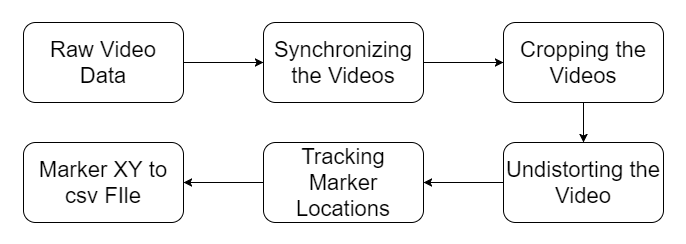
\includegraphics[width=\linewidth]{figures/videoProcess.png}
  \caption{Diagram showing the progression and dependence of the major stages of video processing in the project}
  \label{fig:videoProcess}
\end{figure}

\section{Obtaining Video Data}
Using the chest mounted cameras detailed in the previous chapter we can generate raw video data. The GPHS cameras can be configured to record at different frame rates and resolutions.

%we chose the high 100Hz framerate

%720p by 


\section{Synchronizing Video Sources}
I typical problem faced when working with different sources of data is that of synchronization. Since this project used 4 different cameras, synchronizing the video sources are critical to generate accurate stereo vision data.

The problem of synchronization was overcome by using a audio cue to align the video data post capturing. With all systems recording, a simple hand clap can serve as a spiking audio input easily identified in the audio track of the video streams. The frame associated with this audio spike can be identified using SVP (Sony Vegas Pro) video editing software as shown in the figure below. 

\begin{figure}[!ht]
\centering
  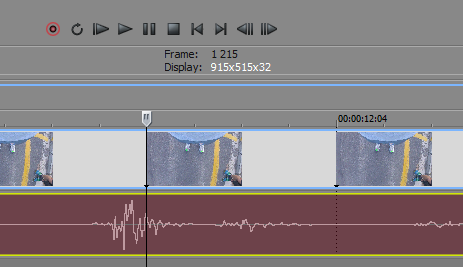
\includegraphics[width=0.5\linewidth]{figures/svpframe.png}
  \caption{Figure showing the user interface of SVP video editing software}
  \label{fig:svpframe}
\end{figure}

The red track in the above figure shows the recorded audio stream while the corresponding frames are displayed in the blue track above that. The cursor is aligned with the audio spike caused by the clap with the corresponding frame number displayed below the playback controls.

This method was repeated for every video stream such that a common starting point was generated. 

\section{Cutting Critical Video Data}

With the video data synchronized the next step was to generate a subset of video demonstrating a transient period and steady state period of running. From accelerometer readings we can easily determine the gait cycle period of our subject; that is the amount of time take between the same foot impacting the ground. These impacts are visible as spikes as seen in the accelerometer data.  

\section{Undistorting the Video Data}
To generate accurate distances using stereo vision the video frames need to be undistorted.

Distortion of the frames is a result of the 

\cite{Hartley2004} 

\section{Tracking and Exporting Marker Positions in the Frame}

using work from \cite{hedrick2008software}











